%!TEX root=../oi-magistr-spolecne.tex
\section[PAL - Grafy - refrezentace a algoritmy]{Neorientované a orientované grafy, jejich reprezentace. Prohledávání grafu (do hloubky a do šířky), topologické uspořádání, souvislost, stromy, minimální kostra.}
Graf je uspořádaná dvojice množiny vrcholů a hran $G = (V,E)$. Dá se reprezentovat mnoha způsoby. Nelze říci, který je lepší, protože se každá reprezentace hodí k trochu jinému typu úloh. Nejčastěji je ale graf reprezentován \textbf{maticí sousednosti} (1 kde je hrana), \textbf{laplaceovou maticí} (na diagonále stupeň vrcholu, -1 pro hranu), \textbf{maticí incidence} (řádky jsou body, sloupce hrany, 1 a -1 značí zdrojový a koncový bod) nebo pomocí \textbf{seznamu sousedů} (u každébo bodu list s jeho sousedama).

\paragraph{Silně souvislá komponenta (SCC)}
Graf je silně souvislý jestliže existuje cesta v obou směrech mezi každými dvěma vrcholy. \textbf{SCC} orientovaného grafu je maximální silně souvislý podgraf.

    $$SCC(v) = \{u \in V |~\text{there exists a path in}~G~\text{from}~u~\text{to}~v~\text{and a path in}~G~\text{from}~v~\text{to}~u\}$$
    
\begin{figure}[h]
    \begin{center}
        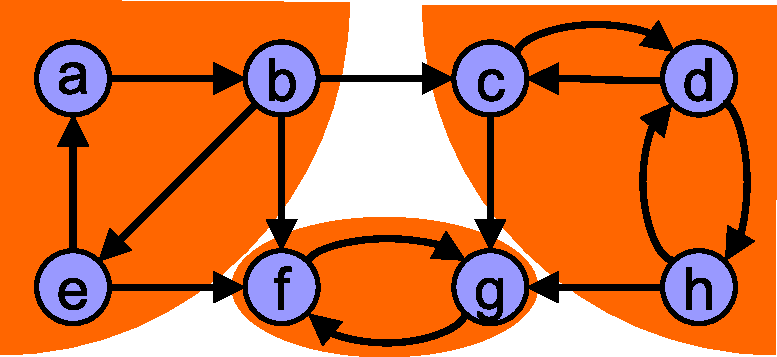
\includegraphics[width=70mm]{02/images/scc}
    \end{center}
\end{figure}

\subsection{Kosaraju}
Používá upravený DFS kde při uzavírání vrcholu ho vloží do stacku $S$. Po prvním průchodu DFS celým grafem prohodí hrany a vyresetuje označení vrcholů. Dokud $S$ obsahuje nějaký vrchol tak ho vybere ze stacku. Pokud vrchol ještě nebyl navštíven tak opět provede DFS. Množina aktuálně navštívených vrcholů dá SCC obsahující i aktuální vrchol.

Algoritmus provádí 2 kompletní průchody grafem. Pokud je graf reprezentován jako list sousedů pak běží v $\Theta(\vert V\vert + \vert E \vert)$, pokud jako matice sousedů tak $O(\vert V^2 \vert)$

\subsection{Tarjan}

Tarjanův algoritmus vychází z prohledávání do hloubky. Vrcholy se při prohledávání indexují dle pořadí svého nalezení. Při návratu z rekurze se každému vrcholu přiřadí uzel s nejnižším indexem na jaký lze dosáhnout. Všechny vrcholy, které mají totožný cílový uzel (index), jsou ve stejné komponentě.

Tarjanův algoritmus má stejně jako prohledávání do hloubky asymptotickou složitost $\Theta(\vert V \vert + \vert E \vert)$ (při použití listu sousedů, jinak při matici sousedů $O(\vert V^2 \vert)$).

\lstset{style=java,caption=Tarjan, label=listing:tarjan}
\begin{lstlisting}
procedure tarjanAlgorithm(Node node, List scc, Stack s, int index)
  v.index = index
  v.lowlink = index
  index++
  s.push(node) //pridej na zasobnik
  for each Node n in Adj(node) do //pro vsechny potomky
    if n.index == -1 //pokud jeste nebyl uzel objeven
      tarjanAlgorithm(n, scc, s, index) //prohledej
      node.lowlink = min(node.lowlink, n.lowlink) //uprav lowlink otce
    else if stack.contains(n) //pokud komponenta nebyla jiz uzavrena
      node.lowlink = min(node.lowlink, n.index)

  if node.lowlink == node.index //pokud jsme v koreni komponenty
    Node n = null
    List component //seznam uzlu dane komponenty
    do
      n = stack.pop() //vyber uzel ze zasobniku
      component.add(n) //pridej ho do komponenty
    while(n != v) //dokud nejsme v koreni
    scc.add(component) //komponentu pridej do seznamu komponent
\end{lstlisting}

\vspace{-15px}

\subsection{Topologické uspořádání}
Topologické uspořádání je taková posloupnost uzlů grafu, že pro každou jeho hranu $(u, v)$ platí, že uzel $u$ je zařazen před uzlem $v$. Topologicky lze proto uspořádat pouze acyklické grafy.

Jinými slovy: Všechny vrcholy grafu G jsou očíslovány tak, že $u\leq v$ platá pro každý pár vrcholů, které mají hranu $(u,v)$

Topologické uspořádání lze zjistit pomocí upraveného DFS. Lze jím testovat grafovou acyklicitu, konektivitu, hledání souvislých komponent.

Algoritmus topologického uspořádání vychází z procházení grafu do hloubky. Jedná se o pořadí uzavření uzlů opačně orientovaného grafu. Časová složitost tohoto postupu proto $O(\vert V \vert + \vert E \vert)$.

\subsection{Minimální kostra grafu - MST}
Kostra grafu G je graf, který má stejný počet vrcholů jako G a je to strom. Minimální kostra grafu je taková kostra, která má součet vah použitých hran nejmenší.

\begin{figure}[h]
    \begin{center}
        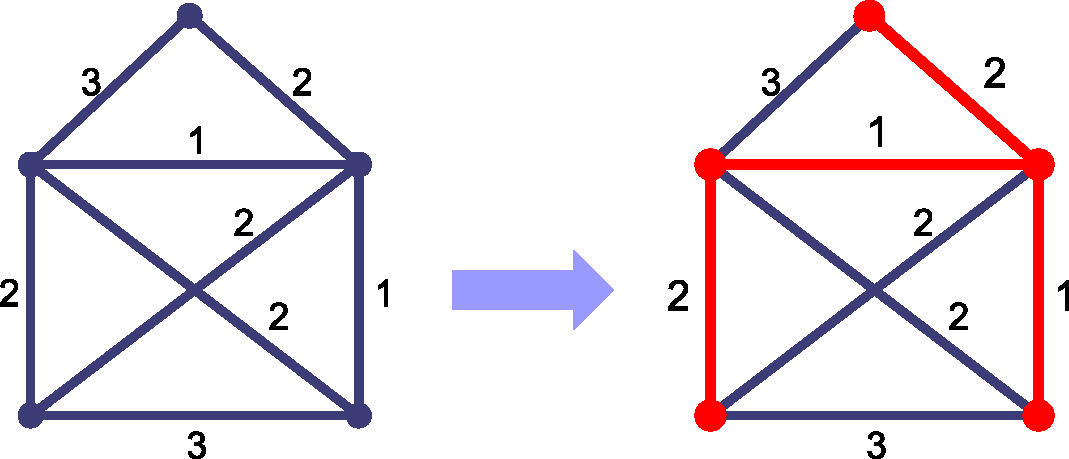
\includegraphics[width=60mm]{02/images/spanning-tree}
    \end{center}
\end{figure}

\vspace{-10px}

\subsubsection{Primův alg.}
Nejprve se vybere libovolný vrchol z $V$ a vloží se do výsledné množiny $K$. K němu se pak v každé iteraci (je jich $V$) hledají takové hrany $(u,v) \in E$, které mají minimální cenu, $u$ je v $K$ a $v$ není v $K$

\begin{algorithm}
\caption{Prim alg.}
\begin{algorithmic}
\State Select an arbitrary vertex $v_0 \in V(G)$
\State $K = \{v_0\}$
\While{$\vert V(K)\vert \neq \vert V(G)\vert$}
  \State Select edge $\{u,v\} \in E(G)$ where $u \in V(K)$ and $v \notin V(K)$ so that $w(\{u,v\})$ is min
  \State $K = K + edge\{u,v\}$
\EndWhile
\end{algorithmic}
\end{algorithm}

\begin{figure}[h]
    \begin{center}
        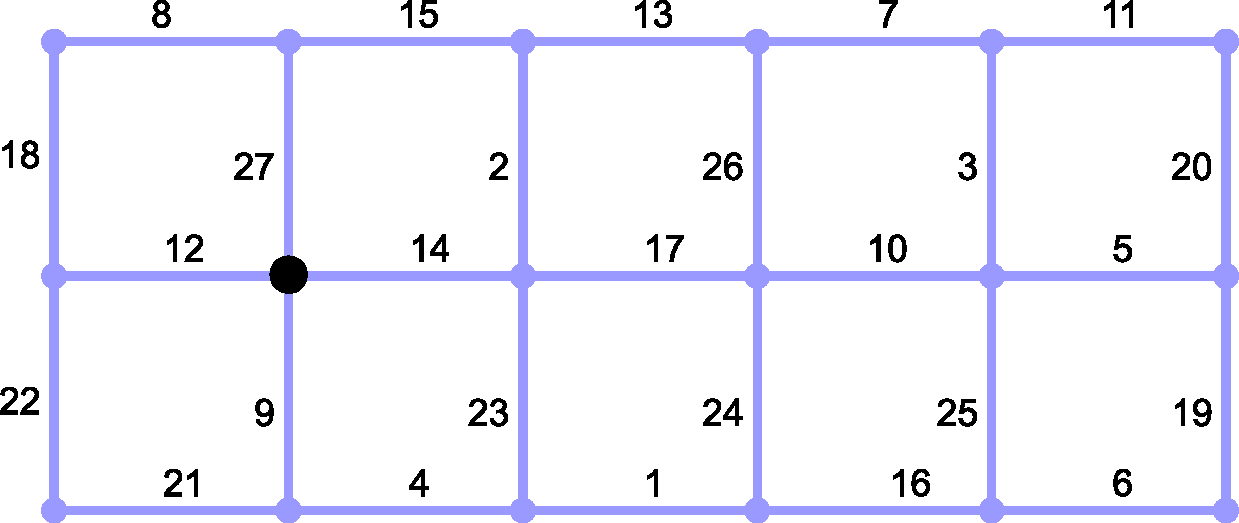
\includegraphics[width=70mm]{02/images/prim01}
        \hspace{10px}
        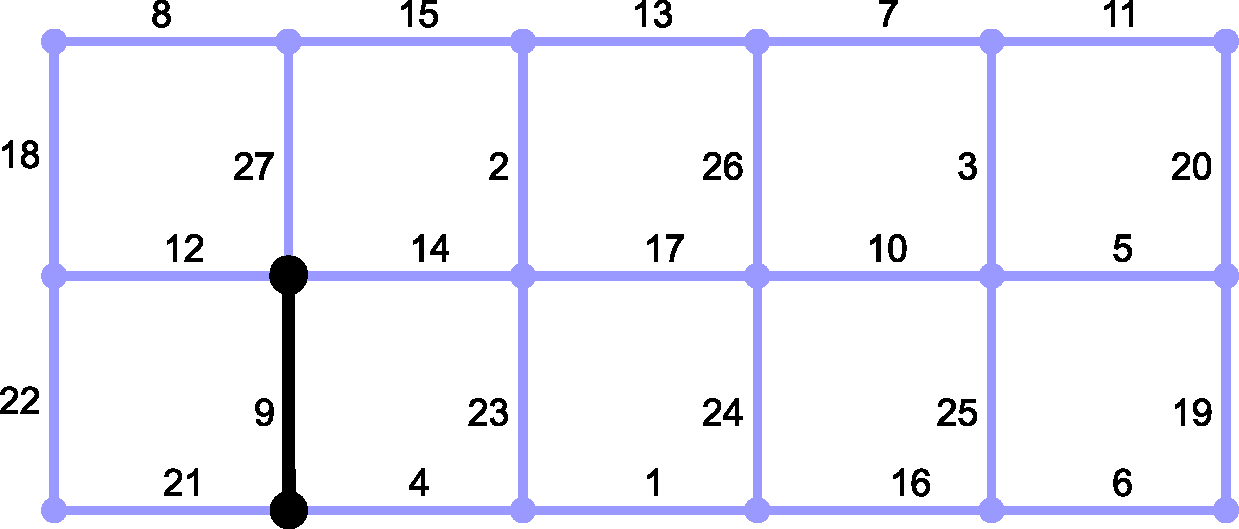
\includegraphics[width=70mm]{02/images/prim02}
    \end{center}
\end{figure}
\vspace{-10px}

Složitost základní implementace je $O(E\cdot V)$. Jednoduchá implementace s použitím reprezentace grafu pomocí matice sousednosti a prohledáváním pole cen má časovou složitost $O(V^2)$. S použitím binární haldy a seznamu sousedů dosáhneme složitosti $O((V + E) \log(V)) = E \log(V)$.


\subsubsection{Borůvkův alg.}
Borůvkův algorimus funguje na principu skládání komponent. Na začátku jsou všechny uzly grafu považovány za samostatné komponenty. Algoritmus v každém svém kroku propojí každou komponentu s jinou komponentou pomocí nejkratší možné hrany. Jelikož Borůvkův algoritmus vyžaduje, aby měly všechny hrany unikátní váhu, tak při propojení komponent nikdy nemůže vzniknout cyklus. Dále je zajištěno, že se v každém kroku zmenší počet komponent minimálně na polovinu - tj. algoritmus terminuje v $\lceil \log_{2} \vert V \vert \rceil$ krocích. Při každém z těchto kroků je třeba najít pro všechny komponenty nejkratší vycházející hranu, což může zabrat až $O(\vert E \vert)$ operací. Celková asymptotická složitost Borůvkova algoritmu je tedy $O(\vert E\vert \cdot \log_{2} \vert V \vert)$.

\begin{algorithm}
\caption{Borůvka alg.}
\begin{algorithmic}
\State $K=(V(G))$
\While{while $K$ has at least two connected components}
  \State For all components $T_i$ of graph $K$ the \textbf{\textit{light incident edge}} $t_i$ is chosen.
  \State All edges $t_i$ are added to $K$
\EndWhile
\end{algorithmic}
\end{algorithm}

\begin{figure}[h]
    \begin{center}
        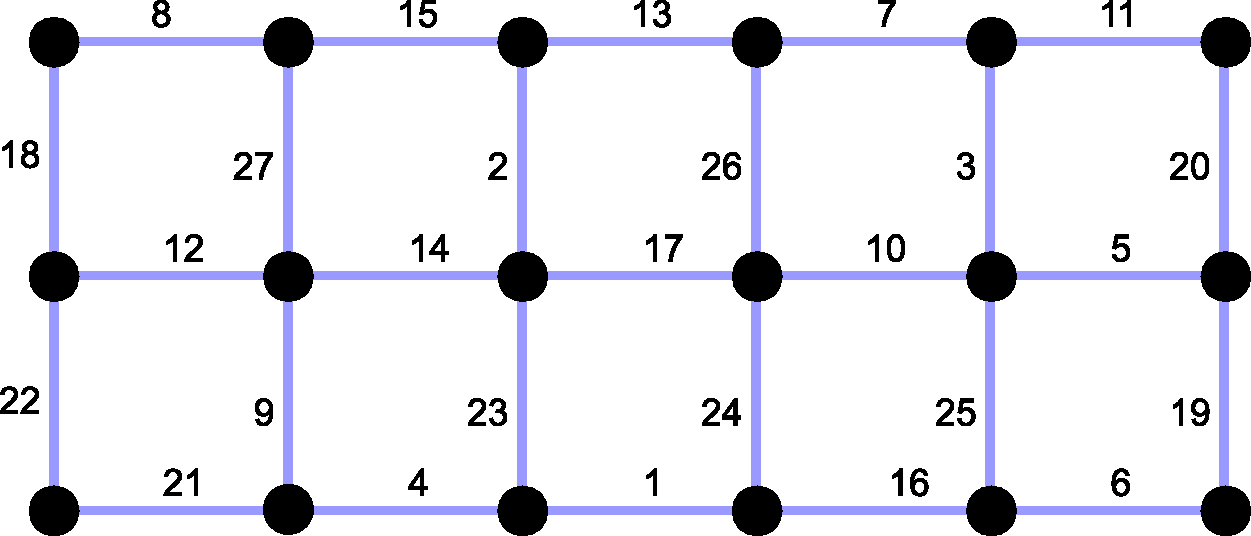
\includegraphics[width=70mm]{02/images/boruvka01}
        \hspace{10px}
        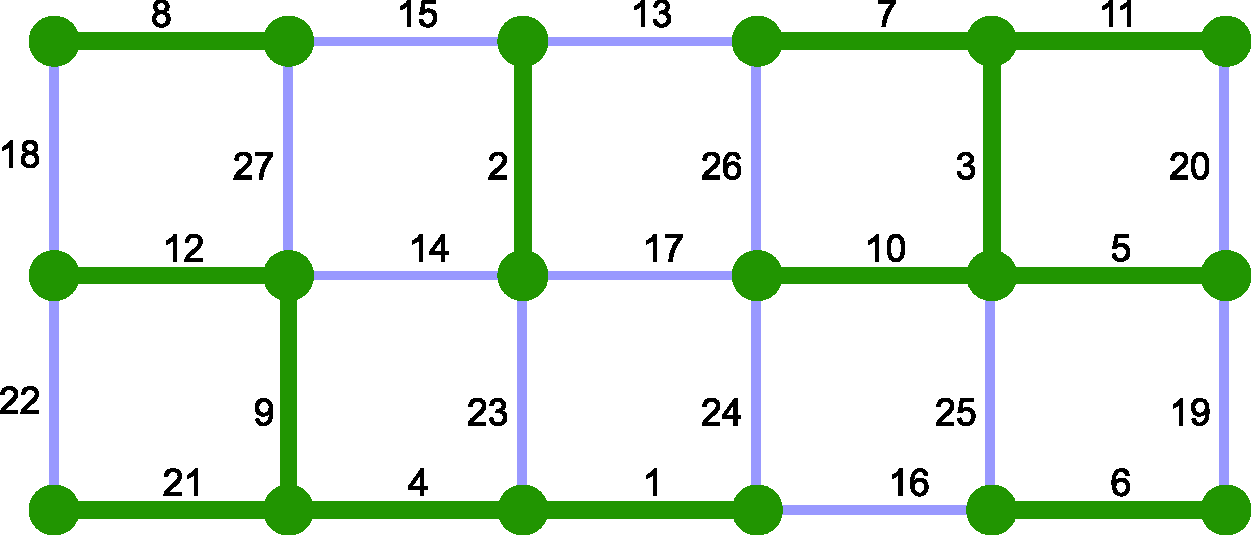
\includegraphics[width=70mm]{02/images/boruvka02}
    \end{center}
\end{figure}

\subsubsection{Kruskalův (\uv{greedy}) alg.}

Kruskalův algoritmus nejprve setřídí hrany dle jejich váhy (od nejmenší) a následně přidává hrany do grafu takovým způsobem, aby nevznikl žádný cyklus (tj. procedura terminuje po přidání $\vert V \vert -1$ hran). V každé iteraci je výsledek podgrafem MST.

K zajištění acykličnosti si algoritmus pomocí datové struktury disjoint set (union-find) udržuje pro každý uzel informaci o příslušnosti ke komponentě souvislosti. Disjoint set poskytuje dvě operace: union (spojí dvě komponenty souvislosti) a find (zjistí pro daný uzel příslušnost ke komponentě souvislosti).

Struktury se ptáme $\vert E(G)\vert$-krát jestli jsou 2 vrcholy ve stejné kmoponentě (operace find) a mergujeme jen $\vert V(G)\vert -1$-krát 2 komponenty do jedné (operace union).

Časová složitost algoritmu je v případě použití řadicího algoritmu založeného na porovnávání $O(\vert E\vert \cdot \log \vert E \vert)$. Pokud jsou hrany již předřazeny, nebo je možno k jejich seřazení použít řadicí algoritmus s lineární složitostí (např. counting sort), tak je složitost Kruskalova algoritmu rovna $O(\vert E\vert \cdot \alpha(\vert E \vert))$, kde $\alpha$ je inverzní Ackermannova funkce (odpovídá složitosti operací union a find).

\begin{algorithm}
\caption{Kruskal alg.}
\begin{algorithmic}
\State Sort all edges $e_1,\dots, e_{m=\vert E(G)\vert} \in E(G)$ so that $w(e_1) \leq \hdots \leq w(e_m)$
\State $K=(V(G))$
\For{$i=1 \hdots m$}
  \If{$K$ + edge $\{u,v\}$ is an acyclic graph}
    \State $K = K$ + edge $\{u,v\}$
  \EndIf
\EndFor
\end{algorithmic}
\end{algorithm}

\begin{figure}[h]
    \begin{center}
        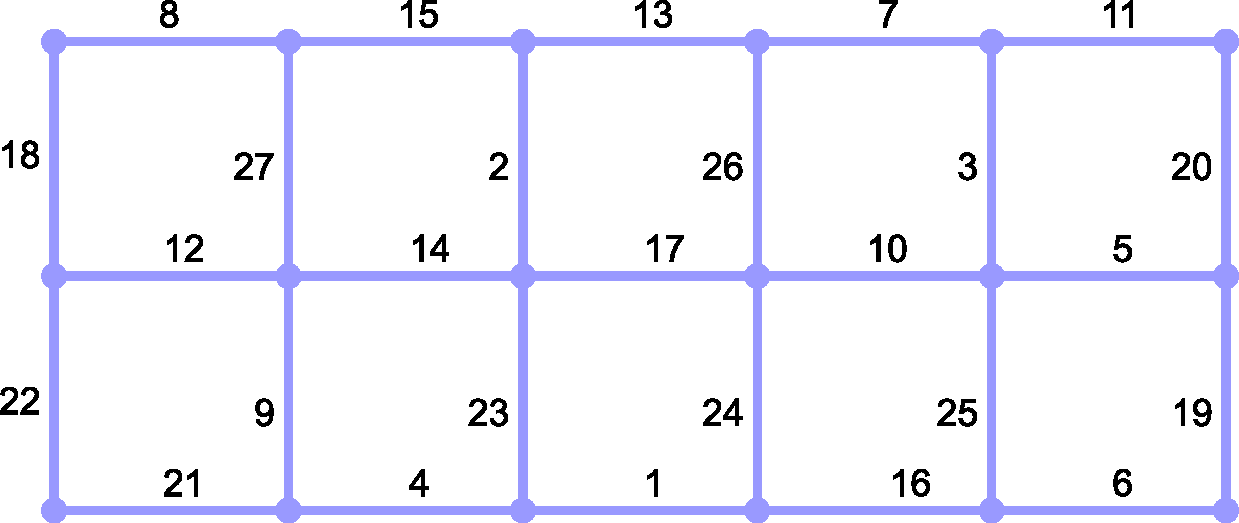
\includegraphics[width=70mm]{02/images/kruskal01}
        \hspace{10px}
        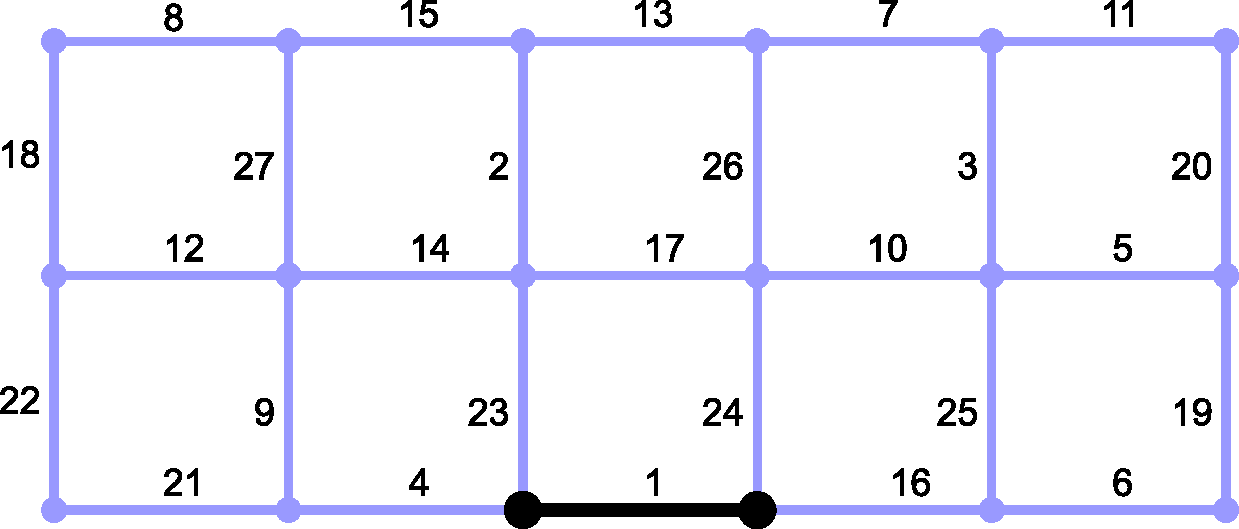
\includegraphics[width=70mm]{02/images/kruskal02}
    \end{center}
\end{figure}

\subsubsection{Union-Find problém}
Problém, který se řeší v kruskalově algoritmu pro hledání MST, při zjišťování, zda 2 vrcholy leží v jedné komponentě, či nikoli - $O(1)$.

\paragraph{Jednoduché řešení} Pole, kde pro každý vrchol udržujem číslo komponenty v jaké je (defaultně obsahuje svoje číslo). Operace find jen vrátí hodnotu na indexu. Union si najde pomocí findu oba prvky a pokud jsou ruzné, tak hodnota jednoho prvků je přepsána na hodnotu druhého (ve všech výskytech) - $O(V)$.

\paragraph{Vylepšené řešení za použití orientovaného stromu}
Ve findu, pokud se naleznou prvky s různými komponentami, tak kořen menšího stromu je přidán jako potomek většího. Hodnoty v poli vždy ukazují na roota komponenty.

\begin{figure}[h]
    \begin{center}
        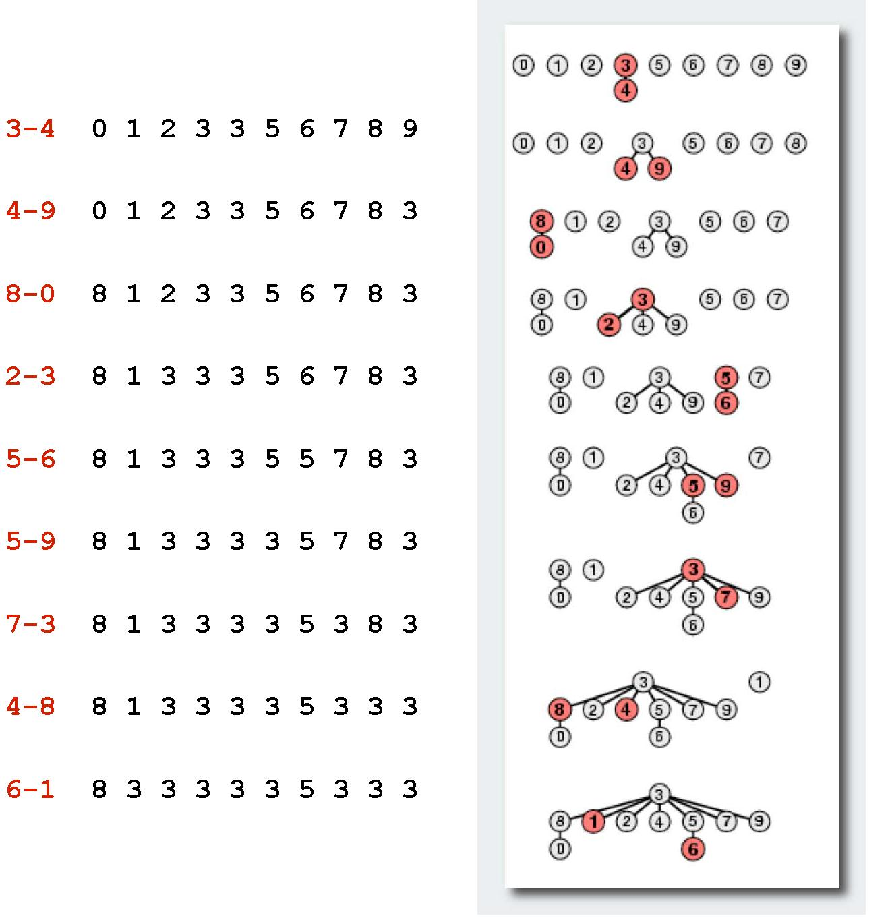
\includegraphics[width=120mm]{02/images/union-find}
    \end{center}
\end{figure}
